%-------------------------------------------------------------------------------
% DRIVEN CAVITY FLOWS 
%-------------------------------------------------------------------------------

\section{2D Driven Cavity Flows} \label{sec:driven_cav}

In two-dimensional (2D) driven cavity flows, a viscous Newtonian incompressible
fluid is confined within a square or rectangular domain. In these model
problems, the fluid is driven by the motion of the bounding walls. The
resulting types of flow configurations have been widely used due to their
simplicity and relevance as benchmark problems for validating numerical solvers
and investigating various flow phenomena.

A recent and comprehensive review conducted by \citet{kuhlmann2019} provides
insights into the extensive research carried out on the many variants of the
lid-driven cavity.

\subsection{The Single Lid-Driven Cavity Flow}

The most basic configuration involves a square cavity where only one wall,
referred to as the lid, is in motion while the other walls remain stationary.
This simple 2D case has been extensively studied numerically and serves as one
of the canonical benchmark problems for numerical Navier-Stokes solvers
nowadays. The first thorough computational investigation lies more than half a
century back \citep{burggraf1966}. Figure \ref{fig:cav_simple} shows the basic
setup, and figure \ref{fig:Re_cav_simple} illustrates typical flow patterns for
two different Reynolds numbers. The depicted streamlines show a central vortex
driven by the upper lid's motion to the right. Therefore, the primary vortex
rotates clockwise. Moreover, the flow shows secondary vortices at the upper and
lower corners at higher Reynolds numbers.

\begin{figure}[ht]
\centering
\begin{tikzpicture}[scale=1.4]
  \draw[thick] (0, 0) rectangle (2, 2);
  \draw[thick, pattern=north west lines, pattern color=gray] (0, 2)
    rectangle (2, 2.15);
  \draw[->, thick] (0.5, 2.25) -- (1.5, 2.25);
  
  \node at (1, 1) {Fluid};
  \node at (1, 2.3) [above] {Moving lid, $U$};
\end{tikzpicture}
\caption{The lid-driven cavity with a tangential velocity $U$ at the top}
\label{fig:cav_simple}
\end{figure}

\begin{figure}[ht!]
\begin{center}
  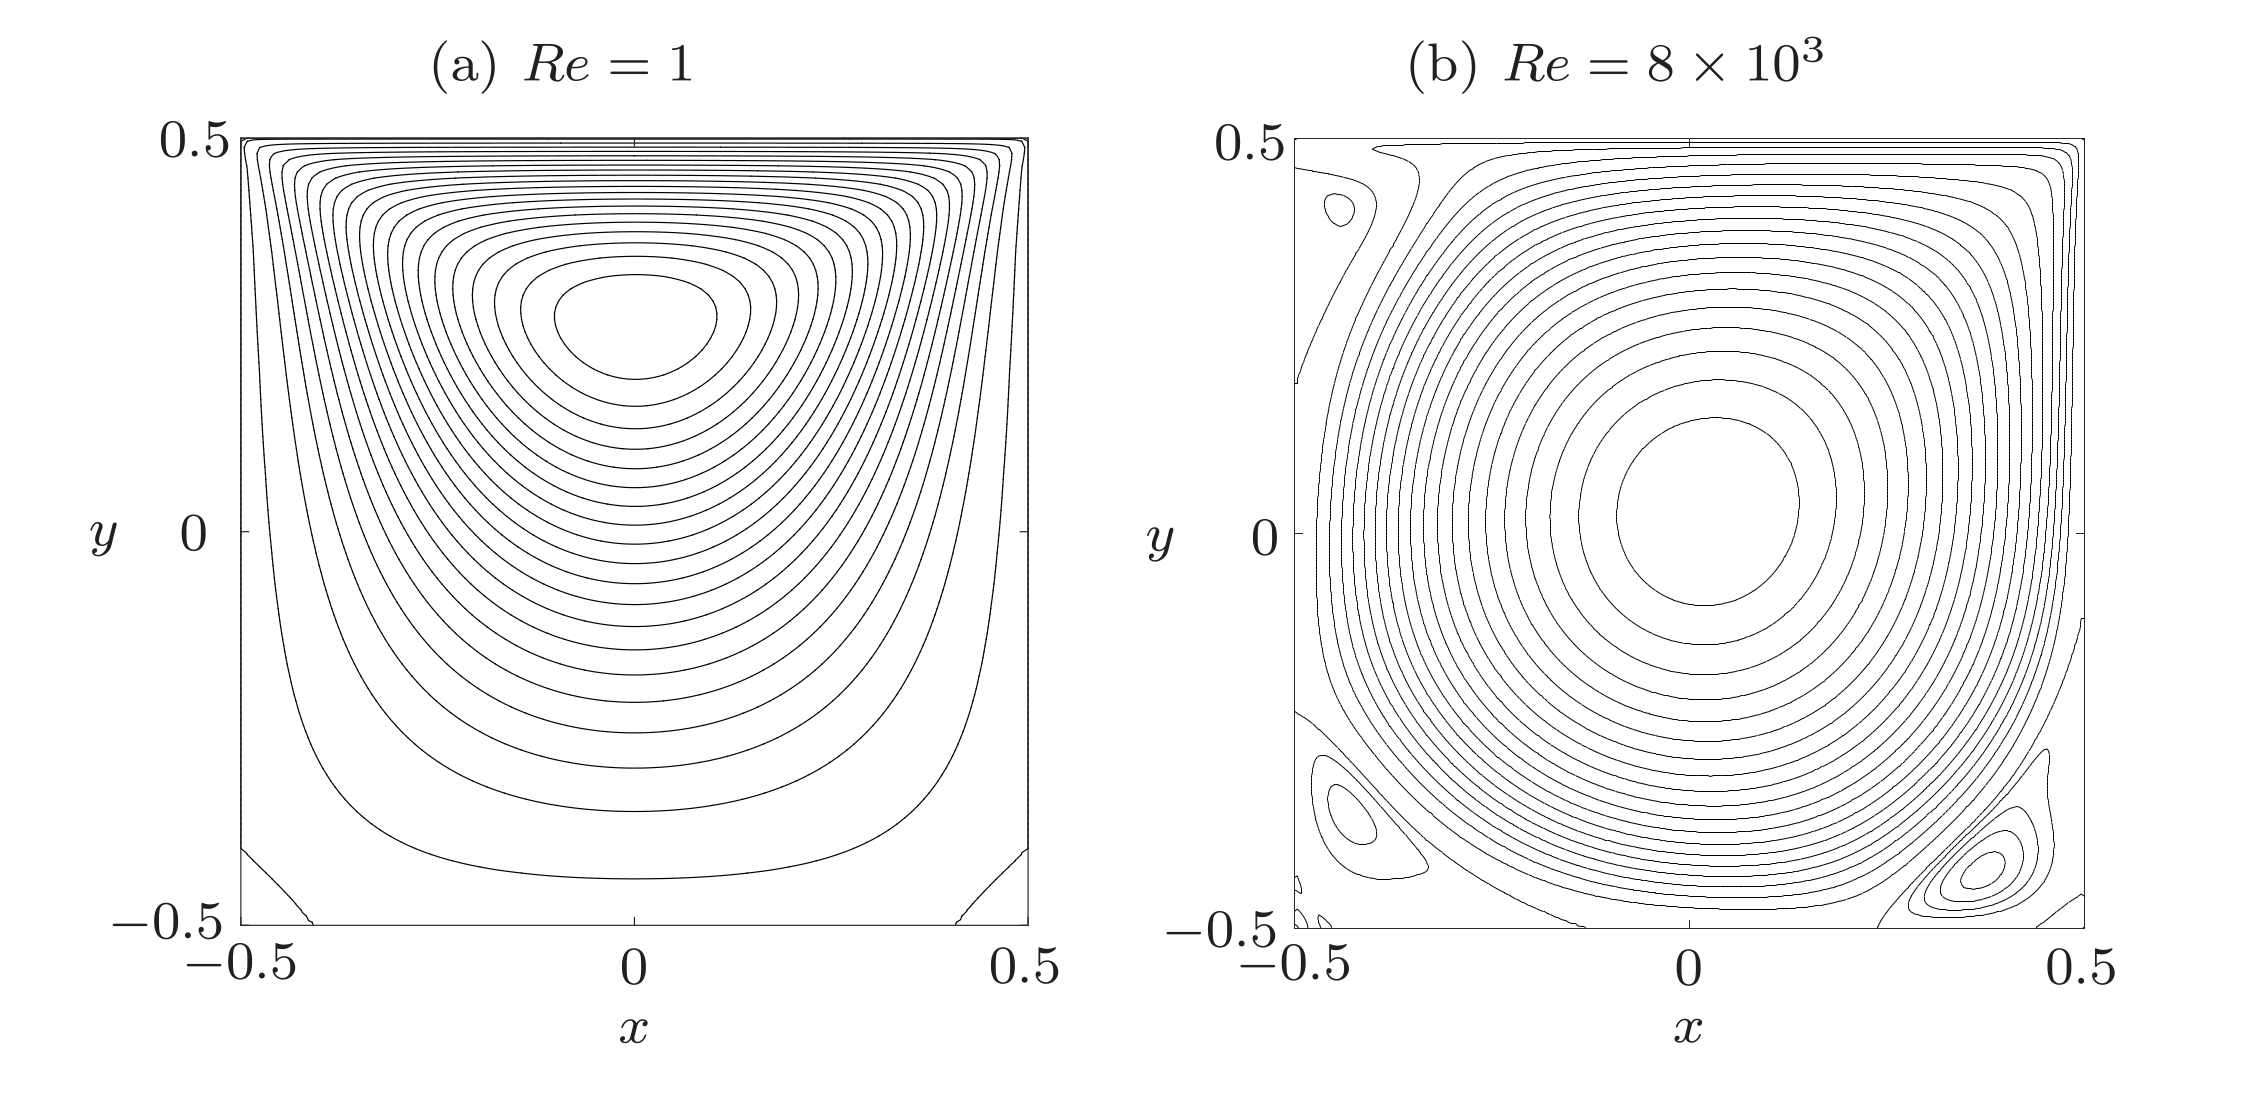
\includegraphics[width=0.65\textwidth]{figs/fig_kuhlmann2019}
\end{center}
\caption{Isolines of the streamfunction of the lid-driven cavity at Reynolds
  numbers 1 (a) and 8000 (b), figures adapted from \cite{kuhlmann2019}}
\label{fig:Re_cav_simple}
\end{figure}

The flow observed in the upper corners is a result of the discontinuous
boundary conditions in the mathematical problem and is caused by the horizontal
component being set to a velocity $U$ at the upper corners, whereas the
vertical walls are not moving. As a consequence, the pressure and the vorticity
diverge at these locations. This phenomenon is a special case of Taylor's
scrapper problem, and there exist closed-form solutions in terms of series
expansions \citep{kuhlmann2019}. The other effect worth mentioning is the
formation of two eddies at the lower corners of the cavity. These vortices
rotate in an anti-clockwise way, separated from the central vortex. They are
called Moffat eddies, and similarity solutions have been found for them
\citep{moffatt1964}.

Apart from these studies, calculating the solutions of the cavity while varying
the Reynolds number has been done extensively. The single lid-driven cavity
becomes unstable at a Hopf bifurcation (see section \ref{sec:bif_details})
somewhere in the range of the Reynolds number [7500, 8100] as reported by
different studies \citep{kuhlmann2019}. No conclusive results could be drawn
due to significant uncertainty. The numerical variations are primarily the
result of the large Reynolds number at which the bifurcations appear and the
different discretizations used when solving the Navier-Stokes equations
numerically. The other issue, as mentioned before, is the corner singularities
caused by the discontinuous boundary conditions.

Until now, we have restricted our attention only to the 2D single lid-driven
case. However, there is a whole spectrum of different variants. The analysis
can be performed for different aspect ratios (height-width ratio of the box),
and one can evaluate the effect on the flow pattern. Shapes other than a
rectangular cavity can be considered as well. With more computing resources
being available, the 3D variant has also been studied, giving rise to other
types of flows and singularities \citep{lopez2017}. Further, the problem can be
combined with heat convection by keeping facing sides at different temperatures
\citep{koseff1985}. \\

In this work, we want to consider another type of flow variant by adapting the
boundary conditions. \cite{kuhlmann1997} investigated a two-sided flow problem
numerically and experimentally where two facing lids move in opposite
directions. It has been found that a primary symmetric flow pattern is stable
for low Reynolds numbers. Then the flow transitions to non-unique patterns and
becomes unstable for higher Reynolds numbers. \citet{wahba2009} did further
numerical experiments in a modified non-facing version of the two-sided cavity
problem. Moreover, an extension was proposed, the four-sided version (figure
\ref{fig:cav_4s}), where all four walls are moving, having the same tangential
speeds but in opposite directions. The figure below illustrates the different
variants for the boundary conditions.

\begin{figure}[ht]
\centering
\begin{subfigure}[b]{0.3\textwidth}
  \centering
  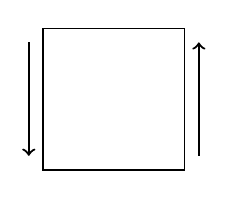
\begin{tikzpicture}[scale=1.8]
    \draw (0,0) rectangle (1,1);
    \draw[thick, ->] (-0.1,0.9) -- (-0.1,0.1);
    \draw[thick, ->] (1.1,0.1) -- (1.1,0.9);
    \draw[thick, ->, color=white] (0.9,-0.1) -- (0.1,-0.1);
  \end{tikzpicture}
  \caption{Two-sided lid-driven cavity \\ \hspace{\textwidth}}
  \label{subfig:bc_2s}
\end{subfigure}
\begin{subfigure}[b]{0.3\textwidth}
  \centering
  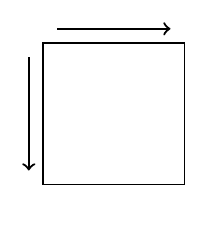
\begin{tikzpicture}[scale=1.8]
    \draw (0,0) rectangle (1,1);
    \draw[thick, ->] (-0.1,0.9) -- (-0.1,0.1);
    \draw[thick, ->] (0.1,1.1) -- (0.9,1.1);
    \draw[thick, ->, color=white] (0.9,-0.1) -- (0.1,-0.1);
  \end{tikzpicture}
  \caption{Two-sided lid-driven cavity (non-facing)}
  \label{subfig:bc_2s_nf}
\end{subfigure}
\begin{subfigure}[b]{0.3\textwidth}
  \centering
  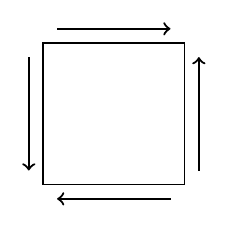
\begin{tikzpicture}[scale=1.8]
    \draw (0,0) rectangle (1,1);
    \draw[thick, ->] (0.1,1.1) -- (0.9,1.1);
    \draw[thick, ->] (1.1,0.1) -- (1.1,0.9);
    \draw[thick, ->] (0.9,-0.1) -- (0.1,-0.1);
    \draw[thick, ->] (-0.1,0.9) -- (-0.1,0.1);
  \end{tikzpicture}
  \caption{Four-sided lid-driven cavity \\ \hspace{\textwidth}}
  \label{subfig:bc_4s}
\end{subfigure}

\caption{Variations of the boundary conditions for the cavity flow,
 with the moving lids set to an equal tangential speed $U$}
\label{fig:bc_types}
\end{figure}

\subsection{\red{The Four-Sided Lid-Driven Cavity Flow}} \label{sec:4sc}

We will focus on the four-sided version of the cavity flow problem. In this
configuration, the top and bottom lids move in the rightward and leftward
directions, while the right and left lids move in the upward and downward
directions, respectively. The dimensional quantities that characterize this
cavity flow are depicted in figure \ref{fig:cav_4s}.

\begin{figure}[ht]
\centering
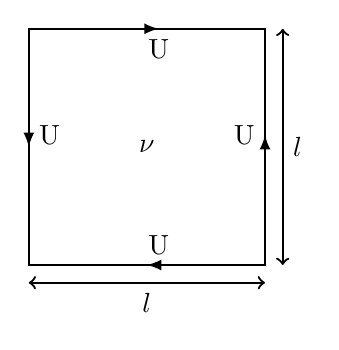
\begin{tikzpicture}[scale=1.5]
  \draw[thick] (0,0) rectangle (2,2);
  \draw[thick] (0,0) rectangle (2,2);

  \node at (1,1) {$\nu$};

  \draw[-latex, thick] (2,0) -- node[pos=0.9, above] {U} (1,0);
  \draw[-latex, thick] (0,2) -- node[pos=0.9, right] {U} (0,1);
  \draw[-latex, thick] (2,0) -- node[pos=1, left] {U} (2,1.1);
  \draw[-latex, thick] (0,2) -- node[pos=1, below] {U} (1.1,2);

  \draw[<->, thick] (0,-0.15) -- node[pos=0.5, below] {$l$} (2,-0.15);
  \draw[<->, thick] (2.15,0) -- node[pos=0.5, right] {$l$} (2.15,2);
\end{tikzpicture}
\caption{The four-sided cavity ($l \times l$) with tangential velocities $U$
  and kinematic viscosity $\nu$ }
\label{fig:cav_4s}
\end{figure}

The study by \citet{wahba2009} reveals the existence of multiple steady
solutions and shows an interesting flow bifurcation at a low to moderate
Reynolds number. Further, this bifurcation happens at an even lower Reynolds
number compared to the two-sided versions. Initially, the global flow pattern
exhibits symmetry, and then two stable asymmetric solutions emerge, whereas the
symmetric solution becomes unstable. The symmetric state consists of four
coexisting vortices, which eventually collapse into two different asymmetric
states of central primary rotations and two secondary vortices. Figure
\ref{fig:4fsc_states} provides a visualization of these states and the rotation
direction of the resulting vortices. The numerical simulations were carried out
on a finite-difference grid using the line successive over-relaxation method
(LSOR). \\

\begin{figure}[ht]
  \centering
  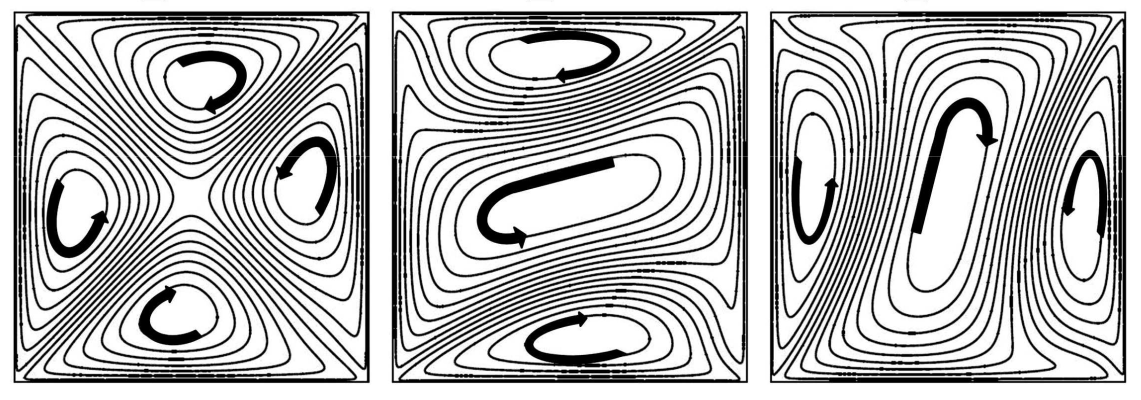
\includegraphics[width=0.6\textwidth]{figs/fig1_chen2013}
  \caption{Symmetric and asymmetric solutions at Reynolds number, $Re=250$,
    computed by \cite{chen2013}}
  \label{fig:4fsc_states}
\end{figure}

Later, \cite{perumal2011} employed a Lattice Boltzmann Method (LBM), recovering
the multiple solutions previously obtained by the former
finite-difference-based code. Furthermore, other aspect ratios for the cavity
have been considered, which exhibit the multiplicity of solutions as well. 

\cite{cadou2012} developed numerical tools for the stability analysis of the
two- and four-sided cavities. They identified a secondary bifurcation point of
the unstable symmetric solution at a higher Reynolds number for the two-sided
non-facing and the four-sided versions. Moreover, a Hopf bifurcation has been
discovered for the two-sided non-facing boundary conditions. On the other hand,
in the four-sided version, no such bifurcation has been reported in the
literature.

A full bifurcation diagram was presented by \cite{chen2013}, which plots the
streamfunction value at the center of the cavity against an increasing Reynolds
number. Through a continuation algorithm, the asymmetric solution branches
could be followed (see section \ref{sec:cont}) and are visualized in the
diagram. The solid curves represent stable solutions, whereas the dashed curves
correspond to unstable ones. One notices that the effect of changing the
Reynolds number in the four-sided version reveals two pitchfork bifurcations
and saddle-node (fold) points for the asymmetric solutions.

The bifurcation diagram generally illustrates that this could be an ideal
bifurcation benchmark. The Reynolds numbers are within a low to moderate
range, making it feasible from a computational point of view. The precise
detection of the two asymmetric solutions can be used to assess the accuracy of
a Navier-Stokes solver under test.

However, it has to be mentioned that the bifurcation diagram was obtained using
a \red{second-order finite differences scheme (non-uniform)}. As pointed out,
the goal here is to look at a regularized problem with the aim of applying a
spectral discretization and accurately resolving the locations of the
bifurcations. To do so, the governing equations will now be introduced
formally, and mathematical well-posed boundary conditions will be defined to
achieve higher accuracy and an exponential convergence rate.

\begin{figure}[h!]
  \centering
  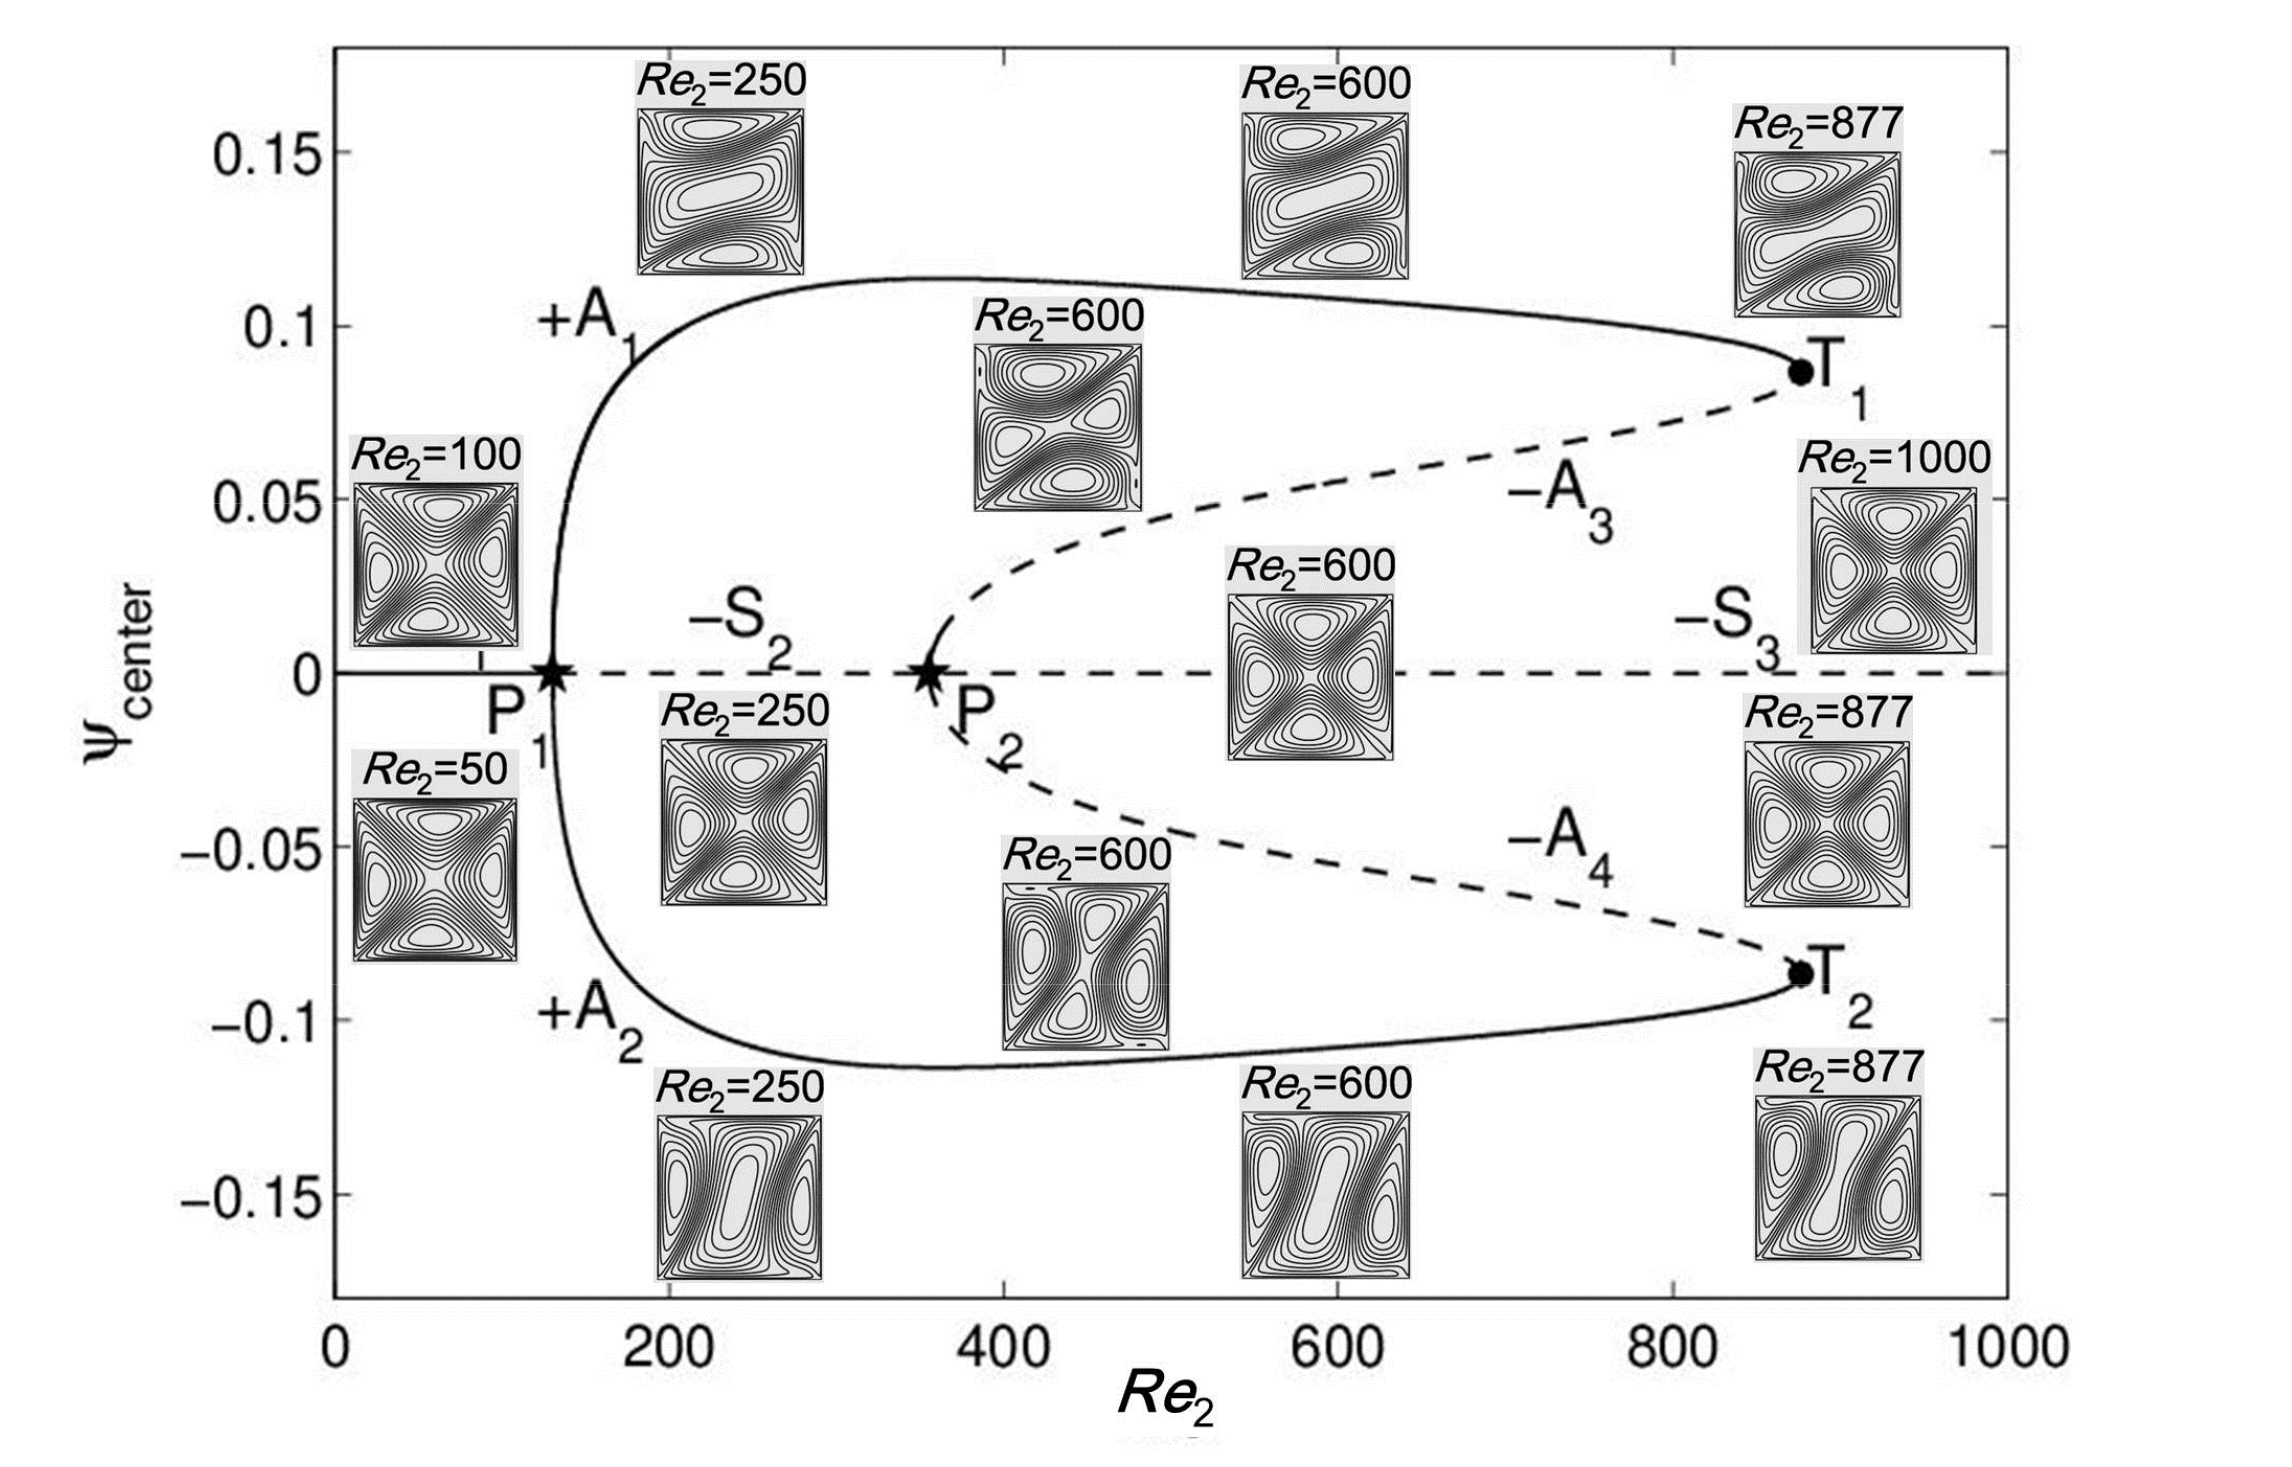
\includegraphics[width=0.85\textwidth]{figs/fig2_chen2013.png}
  \caption{Bifurcation diagram obtained by \cite{chen2013} for the
   four-sided cavity flow, Reynolds numbers are 
    double the results obtained in this study} 
  \label{fig:bif_diag_chen}
\end{figure}

\vspace{100pt}

